% Capitulo 3
\chapter{Validation}\label{validationChap}

To validate our guidelines, we searched for open-source tools that could possibly require database transitions. As stated on Section \ref{introductionChap}, a database migration is justified when the alternatives have better performance/manutenability than the classic RDBMSs and/or the cost to have a similar performance on the relational database architecture is significantly higher.

This condition (assessing the need for a database transition) is, then, only verifiable on production or simulated environments. Wordpress\cite{wordpress}, world's most popular Content Management System (CMS)  \cite{cmsranking}, can be used to illustrate this problem.  

Wordpress is built on the top of relational databases, such as PostgreSQL and MySQL. So, to justify a database transition on a wordpress-based application, we must \textit{(i)} have access to a deployed and active version of the CMS or \textit{(ii)} build a simulated environment and load it with posts, pages, comments and other entities that are present on a regular wordpress website.

Having access to the production version of a heavily used tool, such as Wordpress, is not easy, as the owner of the CMS must give access to sensible information of its database, users and posts. 

Other open source tools were considered on this phase of the research, such as Redmine \cite{redmine} and Moodle \cite{moodle}, but the same problem that emerged trying to accessing sensible information of Wordpress environments was found on these tools.

Besides that, famous open source tools usually have a large user-base. This results in a large support from the community towards the development of the software. With that, if a database transition from RDBMs to NoSQL is needed, it possibly have plugins/addons from the community, as \cite{fantasticElasticsearch}.

Facing this access restrictions to popular open-source projects, to validate the Guidelines proposed on the previous chapter, we have built scenarios that can be easily mapped to real-world applications.

The application proposed on section~\ref{socmediamonitoringapp} is used to illustrate our case studies.

\section{Assessing database transition on a social media monitoring application}
\label{socmediamonitoringapp}

To validate the guidelines presented on Chapter~\ref{theProblemChap} we have modeled \textit{the core database schema} of a social media monitoring  application. Some examples of industry platforms of this kind are \cite{sproutsocial}, \cite{mention} and \cite{buzzmonitor}. 

This category of applications are capable of searching and storing posts from social media platforms, as Twitter and Facebook. On the setup of a new account, users usually define a boolean query of the terms that they want to monitor and the platform begins to monitor \textit{Application Program Interfaces} (APIs) from social networks, searching publications that match the boolean query. 

\subsection{Application Requirements and use cases}
\label{appoperations}
From a user perspective, this kind of application might be used to search for relevant topics across social media posts, to be aware of public opinion about brands (brand awareness) or to assess market for a product, for example. 

From a software engineering perspective, some use-cases of this application could be:

\begin{enumerate}
\item{\textbf{Create, retrieve, update and delete (CRUD) user account} - Users are able to create, modify and delete their account from the application.}

\item{\textbf{CRUD users' terms to monitor} - Users are able to edit the terms that they want to monitor across social networks.}

\item{\textbf{Retrieve posts by ids} - Given a set of post ids, the user is able to visualize them on the user interface (UI).}

\item{\textbf{Classify posts (add/tags tags)} - \textit{N} tags (subjects) can be added or removed from a set of posts.}

\item{\textbf{Filter captured posts by filters} - Some possible filters are: 
\begin{itemize}
\item{Boolean Query:} Search posts that mention a boolean query string. \textit{i.e: (Brazil AND Neymar) OR (Orlando AND Kaka)}
\item{Date:} Search posts that were published within a date range. For example: posts from 2015/01/01 to 2015/02/01.
\item{Tags:} Search posts that match a tag query. i.e: posts about ``Soccer Player'' and ``High Salary''.
\end{itemize}
}

\end{enumerate}

Other possible features and use-cases of this kind of applications are not listed to enable a deeper view of the scenarios that are presented on the next sections.

\subsection{Application Architecture}
Building applications like this one brings some challenges and decisions to software architects and engineers. As the scope of the project grows, it can be a wise decision to split the application in various sub-applications (or components).

Moreover, it is quite costly to manage the whole application from a single code base. The source code needs to handle users registration, query several API's and automatically analyze the sentiment of posts using Natural Language Processing techniques, for example. 

Each of these components may have several other sub-components, or microservices. A microservice architecture brings some benefits to the application, such as maintainability, reuse and simplicity of deployment. A microservice that automatically detects the language from a given a string, for example, can be built and used in all components that need to accomplish this task. 

Components or service-oriented architecture are useful as they enable using different technologies for distinct purposes. Just as in polyglot persistence, the idea is to use the best technology for each task.

Several sub applications could be proposed and created to work with each social network that is supported by the application. For instance, one service/component might be able to handle all the content related to \textit{Facebook}, other component may be responsible for \textit{Twitter} and another one for \textit{Pinterest}-related features. 

On Figure~\ref{fig:apparchitecture} we illustrate a component-based architecture for the proposed application.

\begin{figure}[ht!]
\centering
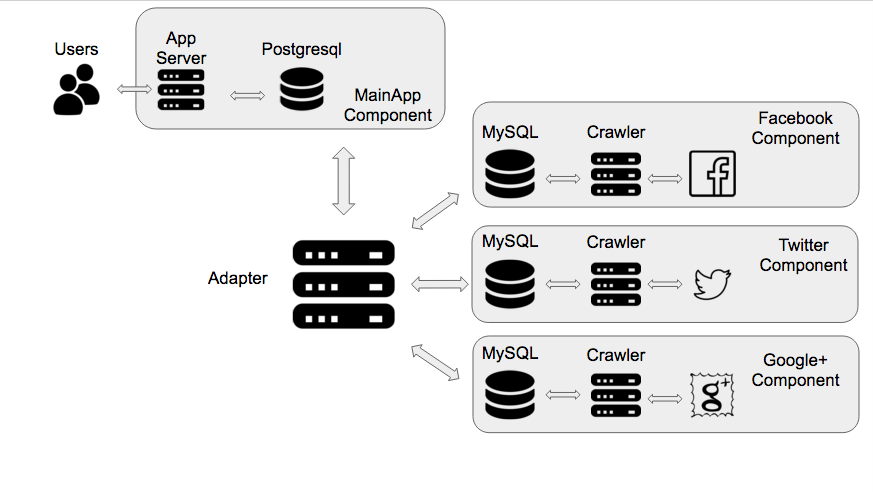
\includegraphics[width=120mm]{Imagens/apparchitecture.png}
\caption{Proposed architecture - Social Media monitoring app.\label{fig:apparchitecture}}
\end{figure}

Five main components can be extracted from the proposed architecture: 

\begin{itemize}
\item{
\textbf{MainApp Component}: This component can be seen as a web application where users can create their account, manage their social profiles, edit the terms that they want to monitor and where the user-interface is presented. A web framework, such as Ruby on Rails or Django can be used to build this component. 
}

\item{
\textbf{Twitter, Google Plus and Facebook Components}: These components are responsible to provide the necessary communication between the MainApp component and Social Networks. The strategy to build a component for each social network was assumed as different social networks have distinct APIs, with different entities and distinct communication patterns.

In other words, \textit{Facebook} may release its API through a HTTP REST perspective, while \textit{Twitter} may release Software Development Kits (SDKs) to a restrict set of programming languages (Gems for Ruby, JARs for Java, for example) and Google plus may release its API through the SOAP protocol, making XML the standard way to handle data on its scenario.   
}
\item{

\textbf{Adapter Component}: The adapter component is responsible to integrate and to act as an interface between the different schemas that compose the data layer from other components (Facebook, twitter and Google Plus).

}
\end{itemize}

As presented on Figure~\ref{fig:apparchitecture}, the architecture of the proposed application relies a Polyglot Persistence strategy. Two distinct databases are used on the app: Postgresql and MySQL. On real-world scenarios, this situation might be caused, for instance, by legacy code or by internal decisions of application architects.


\subsection{When application grows, problems may arise}
\label{shithappens}

Once the application is released, it is desirable that no performance issues are found. Operations executed by application users should be , theoretically, at a acceptable performance level.

In the Facebook component, for example, it is expected to have no performance issues with tens to hundreds of rows stored on the MySQL database. However, worldwide events, as the Soccer World Cup, or national elections, may start to be suddenly monitored, bringing an unusual workload to the components.  

In these cases, or when the application starts to keep track of millions or billions of data records, application performance and user experience may  be dramatically affected if the engineering team have not performed satisfactory load and stress tests.   

Following this scenario, after some months since application release, the number of records on MySQL databases from the three social-networks components may have grown exponentially. A simple query that checked if a column contains a substring would now need to analyze millions of posts instead of hundreds. As the number of posts to be analyzed grows, the query time may also grow.

\subsection{Does the application need other databases?}
\label{anotherdb}
On the scenario described on section~\ref{shithappens}, application users may start to complain that the application is taking too long to process their requests. This situation ends up slowing the overall performance of the users, as an action that should be processed within seconds starts taking minutes to be finish.  

User complains about performance, however, may be related to a number of different factors. To number a few: the business logic might be taking too long to execute, the number of records in the database may have grown in an unexpected way, the database architecture might not be the best choice to handle application data and failures on network or server hardware may exist. 

\textbf{Given this scenario, we will focus our analysis on the components that are responsible for storing the posts on MySQL databases. More precisely, our study will be focused on the Facebook component, to present a clearer definition of the problem.}

A possible complain from the application users' is that the application is getting slower month after month to filter, process and present the posts on  the user interface (UI). 

It is expected that the number of posts grow month after month. In this case, the search speed slows down as the number of posts in the database grows, and application developers and DBAs may use this fact as a hint to start searching for the real cause of the problem. 

This way, the engineering team from the Facebook component might have a strong intuition that the cause of the slowness is on the data layer (MySQL). Engineers may also have an intuition that it is a specific kind of SQL query that is taking too long to execute, consuming too much CPU \& memory resources. The team may also suggest that a NoSQL technology could be a better fit for the use case that is performing below users' expectation. 

In this case, the guidelines proposed on the previous chapter are a good fit, as they are useful to verify if any problems/bottlenecks exist on the database side and to check if a NoSQL architecture could be a better fit to the scenario.


\subsection{The application setup: Server}
\label{appserver}
In this section we detail the server technical specifications that were used to host the data layer of the application that we presented on the previous section. We have selected a \textbf{T2.SMALL} instance from \cite{amazonec2} to host it, as it is a general purpose and low-price instance. T2.SMALL instances feature the following configuration:

\begin{itemize}
\item{High Frequency Intel Xeon Processors with Turbo up to 3.3GHz Burstable CPU, governed by CPU Credits, and consistent baseline performance}
\item{1 vCPU}
\item{12 CPU Credits/hour}
\item{2 GB RAM}
\end{itemize}

\subsection{The application setup: Software}
The following software configuration was installed on the servers: 

\begin{itemize}
\item{Operating System: Ubuntu 14.04.2 LTS (GNU/Linux 3.13.0-48-generic x86\_64)}
\item{Secure Shell}
\item{MySQL Version: 14.14 Distrib 5.5.44, for debian-linux-gnu (x86\_64) using readline 6.3}
\end{itemize}

\subsection{The application setup: Data}
To retrieve the data that is used on the scenarios, we have developed a web crawler that gathers posts from Facebook and store them on our MySQL database. The data was captured from public posts on popular Fan Pages.

A total number of 3.332.534 posts were captured and the Dump file with these posts is available on \cite{dump}. 

\subsection{The application setup: Database schema}
\label{database_schema_section}
The first database schema was built with the intention of being optimized to production environments, and building \textbf{de}-normalized schemas help to leverage application performance, as revealed by \cite{926306}. 

On Figure~\ref{fig:postsTable} it is possible to view all the columns that compose the \textbf{Posts} table. All post entities, like \textit{message} (content of the post), \textit{link} and \textit{number of likes} are present on this table. 

\begin{figure}[ht!]
\centering
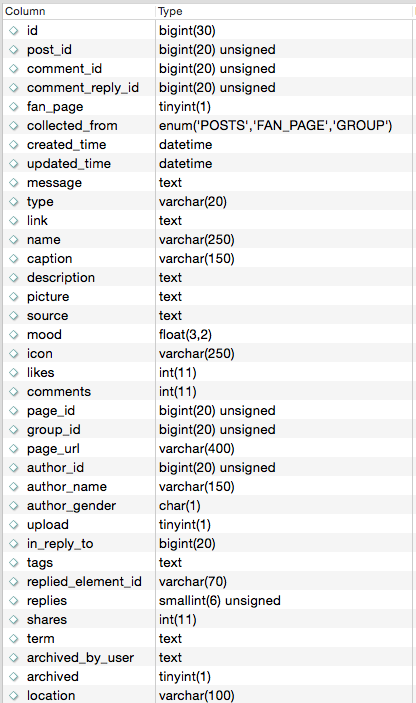
\includegraphics[width=80mm]{postTable.png}
\caption{Posts table.\label{fig:postsTable}}
\end{figure}

Figure~\ref{fig:postsTable} reveals that ``tags'' is a text field on the posts table. By internal convention from the engineering team, a post tag can be represented by a string with a defined format: \textbf{\textit{\#username\_tagname\#}}.

A \textit{tags} cell might store several tags for a single post. Listing \ref{tag_field_standard_format} gives the representation of a tags cell with multiple tags within: 

\begin{lstlisting}[language=json,firstnumber=1, caption=Tag field standard format, label=tag_field_standard_format]
#username1_tag1##username2_tag1##username3_tag1 
\end{lstlisting}

When the user adds a tag to a given post, the ``tags'' field is concatenated with the given tag. A SQL UPDATE that represents this situation is shown on listing \ref{update_tag_sql}.

\begin{lstlisting}[language=sql,firstnumber=1, caption=Update Tag - SQL, label=update_tag_sql]
UPDATE post set tags=concat(tags, '#username3_tag1#') WHERE id=1; 
\end{lstlisting}

To remove a tag, a ``replace'' operator can be used, as shown on listing 

\begin{lstlisting}[language=sql,firstnumber=1, caption=Remove Tag - SQL, label=remove_tag_sql]
UPDATE post SET tags= REPLACE(tags, '#username3_tag1#', '') WHERE id=1; 
\end{lstlisting}

The decision to store the tags in a field instead of storing it on another database was taken to avoid JOINS between several tables when searching for posts that have a set of tags.

\section{Using the guidelines}
As shown on chapter 3, the guidelines proposed on this work are useful to assess and guide database transitions in production-ready or simulated environments. We may use the guidelines to assess if a database migration to NoSQL is really needed or if the problem can be solved by improving the current DB architecture or if it is not even located on the data layer.

Throughout this section we use the guidelines in a step-by-step strategy, as shown on chapter 3, to motivate and guide a database transition on the application proposed on the previous sections of this chapter. 

As stated previously on~\ref{anotherdb}, we want to check if the MySQL Database from Facebook Component needs to be transitioned, given the users are experiencing a degraded QoS in some parts of the application. 

\subsection{List application operations that are performed on database-level}
According to the guidelines, the first step in a scenario where a database transition is being considered is to \textit{List application operations that are performed on database level}. As the focus of our study is the Facebook component, operations from other components, as ``CRUD user account'' and ``CRUD terms to monitor'' should not be considered at this point. 

Thus, from the requirements presented on section~\ref{appoperations}, we identify that the operations that are related to the Facebook Component are \textbf{``Retrieve posts by ids''}, \textbf{``Classify posts (add tags)''} and \textbf{``Filter captured posts by filters''}. These are the operations that could possibly demand a transitioning process on the data layer of the component.  

\subsection{Define user-centered SLAs}

Section \ref{defineusercenteredslas} reveals that for each operation listed on the previous step, a set of SLAs should be proposed. This way, from interviews and surveys with application stakeholders, a network of SLAs could be proposed to the three operations that are subject to our study: 

\begin{itemize}
	\item{\textbf{Retrieve posts by ids}:
		\begin{itemize}
		\item{Ideal threshold: 3 seconds}
		\item{Tolerable threshold: 10 seconds}
		\item{SLA Delta Factor: 3.3X}
		\end{itemize}
	}

	\item{\textbf{Classify posts (add/remove tags)}:
		\begin{itemize}
		\item{Ideal threshold: 1.5 second}
		\item{Tolerable threshold: 3 second}
		\item{SLA Delta Factor: 2x}
		\end{itemize}
	}

	\item{\textbf{Filter captured posts by filters}:
		\begin{itemize}
		\item{Ideal threshold: 3 seconds}
		\item{Tolerable threshold: 10 seconds}
		\item{SLA Delta Factor: 3.3x}
		\end{itemize}
	}

	\end{itemize}

\subsection{Define database-centered SLAs}
As shown on previous sections, users and other application stakeholders are capable of identifying SLAs to the use cases of the application. On the other hand, the application engineers are responsible for defining a set of SLAs that work at database level. 

These SLAs should be \textit{stronger} than the SLAs defined by the users, as several other actions are also necessary to accomplish a single use-case. In the context of a web application, for example, authentication tokens, filters, business logic and network delays are some of the factors that affect the execution time of a use case. 

In this way, a set of Database-oriented SLAs could be defined to the three proposed use-cases: 

\begin{itemize}
\item{
\textbf{Retrieve posts by id}:
	\begin{itemize}
		\item{Ideal threshold: 1.0 seconds}
		\item{Tolerable threshold: 4 seconds}
		\item{SLA Delta Factor: 4x}
		\item{ROFR: 30\%}
	\end{itemize}
}
\item{

\textbf{Classify posts (add/remove tags)}:
	\begin{itemize}
		\item{Ideal threshold: 0.5 second}
		\item{Tolerable threshold: 2 second}
		\item{SLA Delta Factor: 4x}
		\item{ROFR: 30\%}
	\end{itemize}
}

\item{
	\textbf{Filter captured posts by filters}:
	\begin{itemize}
		\item{Ideal threshold: 2 seconds}
		\item{Tolerable threshold: 6 seconds}
		\item{SLA Delta Factor: 3x}
		\item{ROFR: 15\%}
	\end{itemize}
}
\end{itemize}

Thus, from the ``Filter posts captured by filters'' use case, it can be said that a request to filter posts at database level should take up to two seconds to assure that users will not face any performance issues caused by Database-related problems. If the query takes longer than six seconds to execute, users can get really frustrated about the slowness of the tool and this may have a big negative impact on the Quality of Service. 

This SLA also reveals that there should be no problems if up to 15 \% of the requests are executed between two and six seconds. These outlier data points may be caused by expected instabilities on cloud providers. 

\subsection{Build database-level SLA log alerts}

Parts of the application proposed on this chapter were implemented to assess the use of the proposed guidelines. In a real-world scenario, the alerting system could be built within the source code of the application. Other services, such as New Relic, might also be used for this purpose. 

It's also worth mentioning that the SLA checkers are only useful if database queries and processes are actually being executed by the users. In a simulated environment, like this one, user requests can be simulated by load test tools, as JMeter, or can be created programmatically from scratch.

In our case study we proposed and programmatically built scenarios that simulate, at the same time, the requests that are sent by users and part of the source code that analyzes SLA conditions and sends alerts if any SLAs are broken. 

Through the implemented scenarios it is possible to identify if are there any cases where the proposed SLAs are not being fulfilled and consequently if application users may find any degraded QoS caused by database-level problems.

Three scenarios - one for each operation - were built to assess wether the SLAs for each operation are being met or not.

On the following subsections we detail how each scenario was implemented and discuss the motivation to migrate from the relational architecture to a NoSQL strategy on the proposed application. 


\subsubsection{Retrieve posts by id}

The first operation to be checked is to retrieve a set of posts, given their ids. This operation could be originated from a screen that presents a list of posts to the users, where they are able to check for details on each post, for example. 

At database level, this operation can be seen as a simple SQL query, as revealed on listing~\ref{retrieve_posts_by_ids_sql}. 

\begin{lstlisting}[language=json,firstnumber=1, caption=SQL Query - Retrieve posts by ids, label=retrieve_posts_by_ids_sql]
SELECT * FROM posts WHERE id IN (1,2,41,13,12903, ... ,435,31)
\end{lstlisting}\label{query01}

On the previous step, we have defined that a database-level SLA for the \textit{``Retrieve posts by id''} operation is composed by: 

\begin{itemize}
	\item{Ideal threshold: 1.0 seconds}
	\item{Tolerable threshold: 4 seconds}
	\item{SLA Delta Factor: 4x}
	\item{ROFR: 30\%}
\end{itemize}

To verify if the QoS of this operation is below expected, a test environment was setup according to the following steps: 

\begin{enumerate}
\item{For each dataset size on the list [3, 30, 300, 3000, 30000, 300000, 3000000]: }
\item{Retrieve a random number of posts between 50 and 100. These posts are the ones that would be presented to the users;}
\item{Wait for a random time between 30 to 300 milliseconds, to reproduce real-world scenario and avoid	query flood on the database at once;}
\item{Repeat steps 2 and 3 for 30 times for each dataset size.}
\end{enumerate}


Figures \ref{fig:core-execution-01} and \ref{fig:core-execution-01.2} present the Java implementation of the given algorithm. \footnote{This algorithm was run from the database server that host the database to assure that the measured time woud not be affected by network or other hardware-related delays.}


\begin{figure}[ht!]
\centering
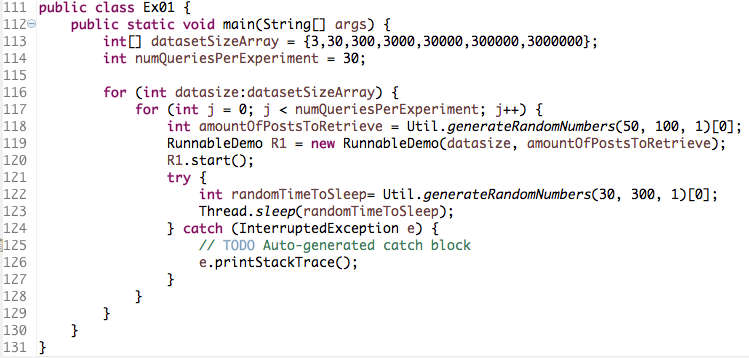
\includegraphics[width=120mm]{Imagens/core-execution-01-1.png}
\caption{Experiment Setup \label{fig:core-execution-01}}
\end{figure}

\begin{figure}[ht!]
\centering
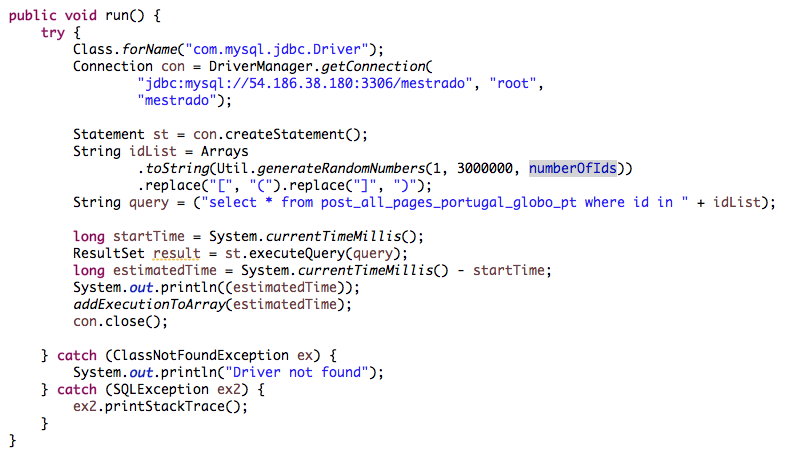
\includegraphics[width=150mm]{Imagens/core-execution-01-2.png}
\caption{Main Thread - Run Method \label{fig:core-execution-01.2}}
\end{figure}


Figure~\ref{fig:core-execution-01.3} presents how the SLA checkers were implemented in Java programming language. As revealed on Chapter 3, alerts are triggered when any query exceeds the tolerable threshold or when the ROFR is above the desired level. We have also defined that a minimum number of 10 operations should be executed before any alert is sent, to avoid unnecessary alerts from unusual situations at the first time that a query is run.

\begin{figure}[ht!]
\centering
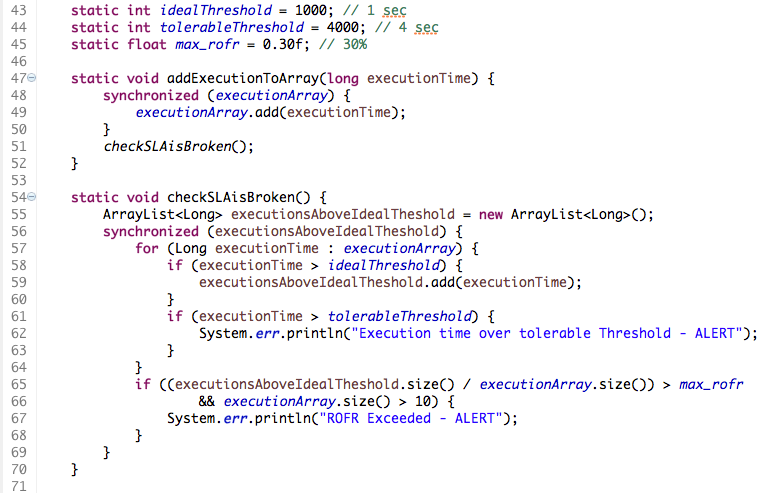
\includegraphics[width=120mm]{Imagens/core-execution-01-3.png}
\caption{SLA Checkers \label{fig:core-execution-01.3}}
\end{figure}


Figure~\ref{fig:first_scenario} shows the execution time in milliseconds for the first scenario. On the chart, each line represents a dataset size, where 30 SELECT queries are sent to the MySQL database and the response time is registered on each query.

\begin{figure}
\centering
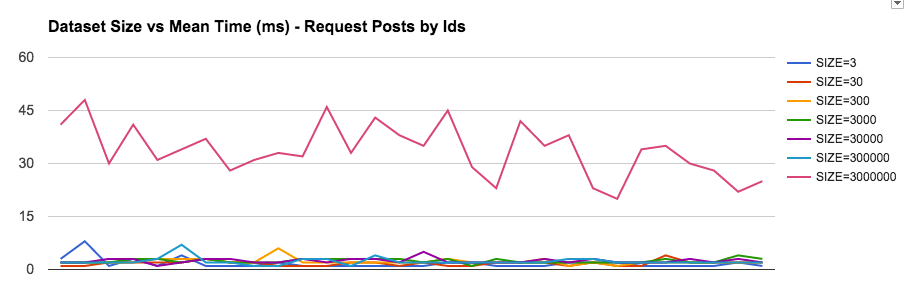
\includegraphics[width=150mm]{Imagens/execution-01.png}
\caption{First Scenario - Retrieve post by ids.\label{fig:first_scenario}}
\end{figure}

As the ideal threshold to this operation states that all operations must be executed in up to 1000 milliseconds (a second), we can assure that the data layer is not a bottleneck to the users on this kind of operation. It is worth mentioning that over 200 queries were executed on this scenario, and not a single query was over 1/10 of the desired ideal threshold.

On the Appendix~\ref{executionreport02} it is possible to visualize the raw data extracted from this scenario. 

\clearpage
\subsubsection{Classify posts (add/remove tags)}

The operation of classifying posts is used when a user wants to add or remove a set of tags from a set of posts. Posts may be updated using their ids or using other tags as references. In other words, it is possible to add or remove a tag from posts that have already been tagged with other tags. In practical terms, the user may want to add a ``SPECIAL\_CUSTOMER'' tag to posts that have already been tagged as ``FAMOUS\_PEOPLE'' or ``RICH\_PEOPLE'', for example. 

Section \ref{database_schema_section} presents how tags may be added or removed from posts in the proposed database schema. Listings \ref{update_tag_sql} and \ref{remove_tag_sql} present a detailed view on how these operations can be performed. 

On the previous section we have defined that a database-level SLA for the \textit{``Classify posts (add/remove tags)''} operation. It is composed by: 

\begin{itemize}
	\item{Ideal threshold: 0.5 second}
	\item{Tolerable threshold: 2 second}
	\item{SLA Delta Factor: 4x}
	\item{ROFR: 30\%}
\end{itemize}

To verify if the QoS of this operation is below expected, a test environment was setup according to the following steps

\begin{enumerate}
\item{For each dataset size on the list \{ 3, 30, 300, 3000, 30000, 300000, 3000000\}:}
\item{Randomly generate a number of tags between 1 and 4; \label{randtags}}
\item{Execute SQL UPDATEs to add one more tag to posts that already have one of the tags generated on step \ref{randtags}.\footnote{If four tags are generated, for example, the SQL statement has the following format: \textit{``UPDATE posts set tags=concat(tags, \#username9\_tag4\#) WHERE tags LIKE \#username6\_tag3\# OR tags LIKE \#username0\_tag7\# OR tags LIKE \#username0\_tag2\# OR tags LIKE \#username0\_tag8\#''}}}
\item{Wait for a random time between 30 to 300 milliseconds, to reproduce real-world scenario and avoid	query flooding on the database at once.}
\item{Start another thread of the same type until a total number of 30 threads are run per dataset size.}
\end{enumerate}

The Java implementation of the proposed environment is presented on Figures \ref{fig:tags-java-01} and \ref{fig:tags-java-02}. The SLA checker for this scenario is very similar to the one that was presented for the first scenario (Retrieve a list of posts by ids) - Figure~\ref{fig:core-execution-01.3}.


\begin{figure}[ht!]
\centering
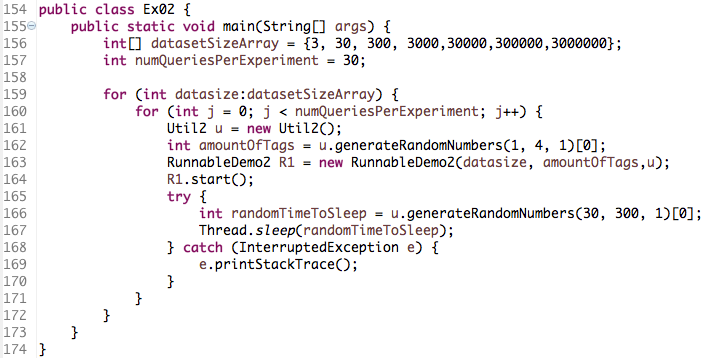
\includegraphics[width=100mm]{Imagens/tags-java-01.png}
\caption{Second Scenario - Add or Remove tags.\label{fig:tags-java-01}}
\end{figure}

\begin{figure}[ht!]
\centering
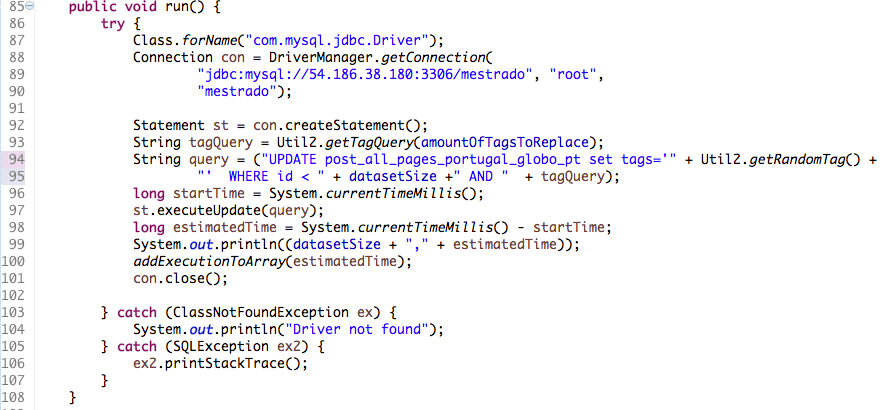
\includegraphics[width=100mm]{Imagens/tags-java-02.png}
\caption{Edit Tags - Run method.\label{fig:tags-java-02}}
\end{figure}

\textbf{Finding a broken SLA}
\hfill \break
The chart displayed on Figure \ref{fig:tags-scenairo-02-chart} shows how the execution time changes (in milliseconds) for this operation between query sizes. 

As can be noticed on the chart, no tolerable threshold is broken or ROFR is exceeded on the datasets from 3 to 30.000 posts. The SLA is eventually broken when querying the datasets sizes are over 300.000 posts. In production environments, this means that the application would work fine on a small scale, but would get sluggish as the database grows.

Big datasets, as the ones over 300.000 posts, present a linearity on the chart. This happens because the jobs are being queued and can only be processed after a previous job finished. Figure \ref{fig:queryQueuing} shows how job queueing is viewed from MySQL's processlist.  

\begin{figure}[ht!]
\centering
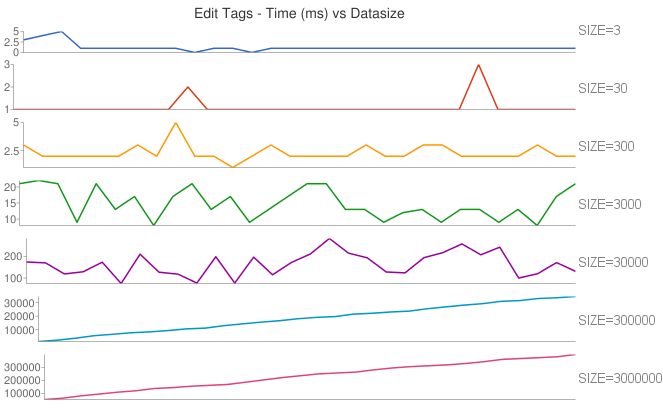
\includegraphics[width=150mm]{Imagens/second-scenario.png}
\caption{Edit Tags - Dataset Sizes vs Time (ms).\label{fig:tags-scenairo-02-chart}}
\end{figure}

\begin{figure}[ht!]
\centering
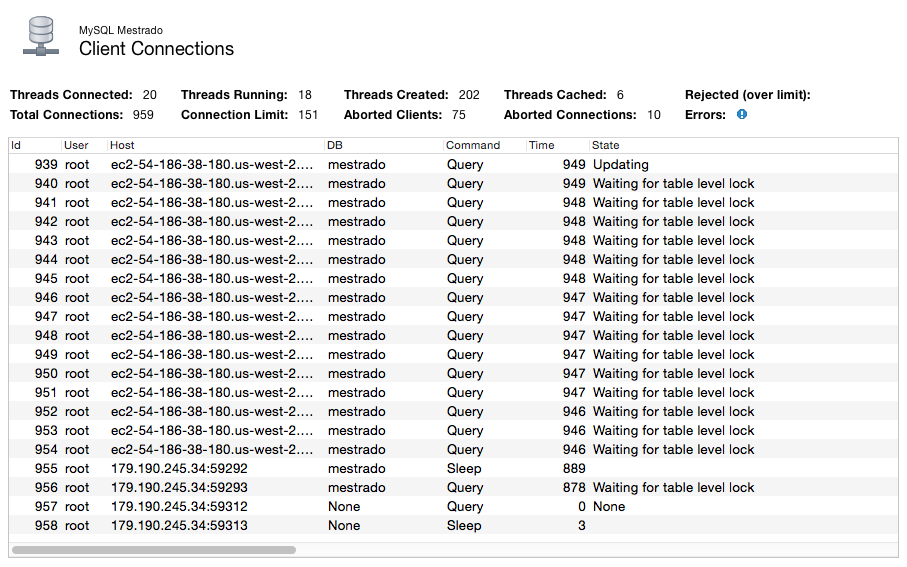
\includegraphics[width=120mm]{Imagens/queryQueueing.png}
\caption{MySLQ Job Queueing.\label{fig:queryQueuing}}
\end{figure}

At this point, we have a broken SLA for the operation.

\clearpage

\subsubsection{Filter captured posts by filters}
\label{filterposts}

The operation of \textit{filtering captured posts by filters} is used when a user wants to visualize only a set of posts that match a defined criteria. Some possible filters are: Sentiment (Positive, Negative and Neutral) - represented on the table as \textit{mood} (a float from 0 to 1, representing the result of a sentiment classifier), \textit{Boolean Query} (words that are mentioned on the post) and Starting Date. \textit{Tags} could also be used as filters at this point, as the previous section suggests. 

Filtering posts at a database level can be represented by a simple SQL query, as illustrated on Listing~\ref{filter-posts-query-example}.

\begin{lstlisting}[language=SQL,firstnumber=1, caption=Filter posts query - Example, label=filter-posts-query-example]
SELECT * from post WHERE mood>0.0 AND created_time > 2015-5-3 AND created_time < 2015-7-15 AND message like '%ruim%'
\end{lstlisting} 


On the previous sections we have also defined that a database-level SLA for the \textit{``Filter captured posts by filters''} operation. It is composed by: 

\begin{itemize}
	\item{Ideal threshold: 2 seconds}
	\item{Tolerable threshold: 6 seconds}
	\item{SLA Delta Factor: 4x}
	\item{ROFR: 15\%}
\end{itemize}

To verify if the QoS of this operation is below expected, a test environment was setup according to the following steps

\begin{enumerate}
\item{For each dataset size on the list \{ 3, 30, 300, 3000, 30000, 300000, 3000000\}:}
\item{Randomly generate a set of filters for date, sentiment (mood) and a Boolean Query;}
\item{Execute SQL SELECTs to retrieve the posts that match the boolean query.}
\item{Wait for a random time between 30 to 300 milliseconds, to reproduce real-world scenario and avoid	query flooding on the database at once.}
\item{Start another thread of the same type until a total number of 30 threads are run per dataset size.}
\end{enumerate}


\textbf{Finding a broken SLA: }
Figure \ref{fig:filter-captured-posts-by-filters} presents how the execution time changes (in milliseconds) for this operation between query sizes. In our implemented scenario, we could also find that there's no noticeable difference between querying random generated ascii-chars and words that actually exist on the posts or on the dictionary.

\begin{figure}[ht!]
\centering
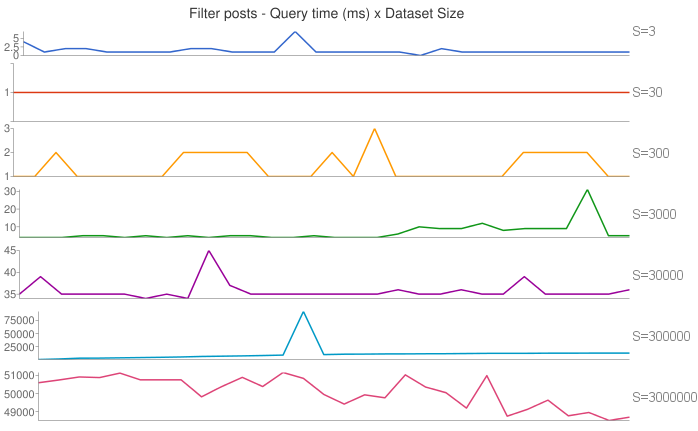
\includegraphics[width=120mm]{Imagens/filter-posts-query-time.png}
\caption{Filter captured posts by filters - Dataset Sizes vs Time (ms).\label{fig:filter-captured-posts-by-filters}}
\end{figure}

As presented on Figure \ref{fig:filter-captured-posts-by-filters}, the SLA for this operation is broken in the same dataset sizes where the operation \textit{Classify posts (add/remove tags) broke, as the numbers on the left represent the time in milliseconds that took for an operation be executed.  }

At this point, we also have a broken SLA for this operation. 























\clearpage
\subsection{Verify SLA violation}
SLA Violations were found on the \textit{Classify posts (add/remove tags)} and \textit{Filter captured posts by filters} operations. 

To find the reason \textit{why} SLA violations were being triggered in these cases, we started by reading performance-related MySQL guides, running EXPLAIN queries and analyzing table columns to check if any improvements could be done on this side.

\subsubsection{Classify posts (add/remove tags)}
\label{classifypostssection}
For this operation, it was clear that the UPDATE was taking too long because it had to scroll over several records to \textit{i) find posts that matched the desired tag query} and \textit{i) perform a row-by-row update}.

MySQL documentation presents other options to perform Full Text Searches rather than using the ``LIKE'' clause. Particularly, a ``MATCH AGAINST'' clause can be used instead of a ``LIKE'' clause to search for tags in this step, as the ``tags'' column is stored as plain text. 

Listing \ref{new-sql-operator-match-against} shows how the two queries differ from each other and \cite{stackoverflowmatch} presents some advantages in using MATCH AGAINST instead of LIKE.

\begin{lstlisting}[language=SQL,firstnumber=1, caption=A new operator - MATCH AGAINST, label=new-sql-operator-match-against]
UPDATE post set tags = "#user1_tag2#" where tags LIKE "#user1_tag1#" -- old sentence
UPDATE post set tags = "#user1_tag2#" where MATCH(tags) against ("#user1_tag1#" IN BOOLEAN MODE) -- new sentence
\end{lstlisting} 

Our DB schema was built using InnoDB Engine, native database engine for MySQL. InnoDB, however, does not support the MATCH AGAINST operator / Full Text Search features \cite{ftsmysql}, so we had to migrate the posts table engine to MyISAM to try the MATCH AGAINST operator. With only 3 million posts stored on our database, the migration lasted for minutes. Migrating a cluster with hundreds of millions of rows in production seems to be a challenging problem. 

MyISAM also has major downsides, however, as revealed by MySQL's documentation: 
\begin{itemize}
\item{No foreign keys and cascading deletes/updates}
\item{No transactional integrity (ACID compliance)}
\item{No rollback abilities}
\item{Row limit of 4,284,867,296 rows (232)}
\item{Maximum of 64 indexes per row}
\end{itemize}
	

After running the same scenario with the MATCH AGAINST operator, the database SLA was still not being met. As advised by \cite{stackoverflowmatch}, this solution quickly becomes unusable for hundreds of rows. 

This way, the literature review proceeded and a possible solution was emerging: to change data format. On the next section we present how changing the data format for tags helped to solve the problem.  



\subsubsection{Filter captured posts by filters}
The issue found on the \textit{Filter captured posts by filters} operation was similar to the one found on \textit{Classify posts}. Indexes were added to the \textit{created\_at} and \textit{mood} columns, and a EXPLAIN query showed that the bottleneck of the operation was to perform a full-text search across several records. 

When the filters were wide, a full table scan was still needed. To ease  understanding, on section \ref{changing-fulltext-search} we present how using the MATCH AGAINST operator together with FULLTEXT indexes \textit{apparently} solved the performance issues of this operation. 













\clearpage
\subsection{Propose architectural changes at database-level}

On the last section, a set of improvements were made to the posts table, but some operation SLAs remained broken. On this section we discuss how changes on the app/database infrastructure could help to fix the broken SLAs.

\subsubsection{Changes on tags structure}
To solve the problem of adding/removing tags to a set of posts that already contain other set of tags, we have proposed a separate table to store tags information. 

Figure~\ref{fig:tagTable} shows the elements that compose a \textit{tag} record. Each tag has a unique ID - \textit{idtags}, a \textit{post\_id} (foreign key to the post table), a \textit{tag\_user} (the username of the user who has tagged this post) and \textit{tag\_name}, the subject of this post. 

The tags table is also denormalized, as \textit{tag\_user} and \textit{tag\_name} are entities that could be represented on separate tables on a normalized schema.

\begin{figure}[ht!]
\centering
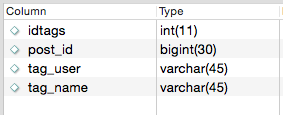
\includegraphics[width=60mm]{tagTable.png}
\caption{Tags table.\label{fig:tagTable}}
\end{figure}

Indexes were added to the \textit{post\_id}, \textit{tag\_user} and \textit{tag\_name} columns. With the proposed table structure, adding and removing tags from a set of posts that have other tags needed new query fomats, as presented on listing \ref{new-sql-queries}.

\begin{lstlisting}[language=SQL,firstnumber=1, caption=New SQL queries to add and remove tags, label=new-sql-queries]

INSERT INTO tags (post_id, tag_user,tag_name) SELECT t.post_id, "newTagUser", "newTagName" from tags t where (t.tag_user= "user1" and t.tag_name="tag1") OR (t.tag_user="user2" and t.tag_name="tag2") -- Create tags 

DELETE FROM tags where (tag_user="user1" AND tag_name="tag1") --Remove Tags

\end{lstlisting} 


The time to create tags in big datasets was, however, still very high, and a set of composed indexes were created on this table. Figure \ref{fig:tagsIndexes} presents all database indexes that were created on the table. Indexes composed by \textit{post\_id}, \textit{tag\_name} and \textit{tag\_user} were essential to leverage performance on the operations. 

\begin{figure}[ht!]
\centering
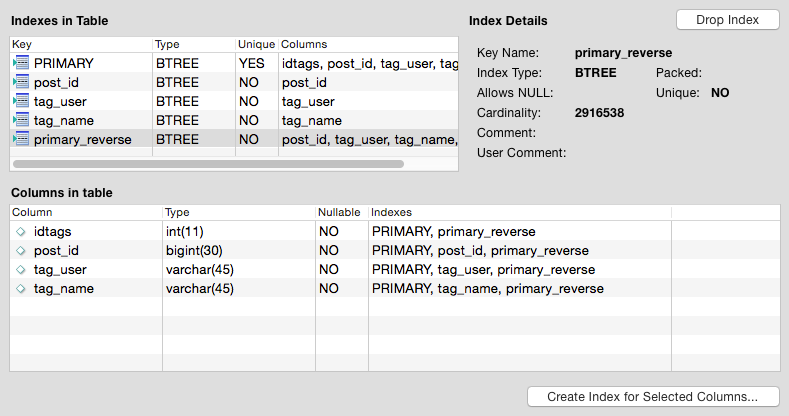
\includegraphics[width=120mm]{Imagens/tagsIndexes.png}
\caption{Tags table Indexes. \label{fig:tagsIndexes}}
\end{figure}

To add tags to posts that already have a set of tags, two actions are necessary: i - \textit{To find} the posts that already have the tags and ii - \textit{to actually write} the tags on the DB. These two steps are also the same for tags removal.

The tags table performance dramatically improved - and made possible - \textit{ to find} posts that already have a set of tags, as presented on Figure \ref{fig:tagsVSposts}.

\begin{figure}[ht!]
\centering
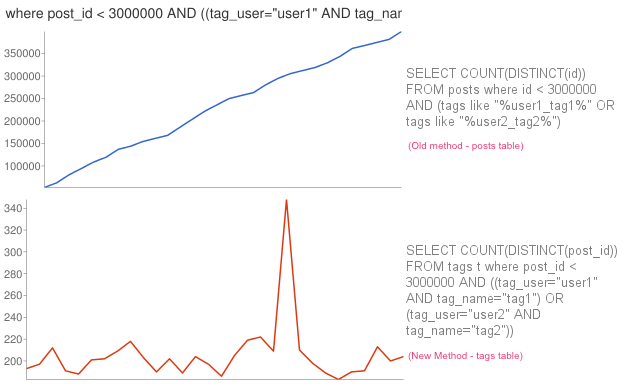
\includegraphics[width=120mm]{Imagens/tagsVSposts.png}
\caption{Retrieve posts to be modified -  (on Tags table / MyISAM) vs Retrieve posts to be modified (on posts table / InnoDB) - 3 million posts dataset.\label{fig:tagsVSposts}}
\end{figure}

It is still not possible, however, to say that the SLA is being respected, as the SLA makes no restriction about how many tags may be added or removed in a single operation. As any Database server has a limited number of operations that it is capable of processing in a period of time (ops/sec), it is not possible to say that a single server will be able to handle the insertion of an infinite amount of tags. 

\textbf{This may evidence that either the SLA needs to be renegotiated with stakeholders or that further work is still needed.} If the renegotiation is possible, users may agree to specify this SLA in terms of the number of tags that can be added/removed per second. i.e: Users may agree that 10.000 tags/second is a satisfiable level. 

If the SLA can't be renegotiated, a possible strategy is to setup a MySQL cluster with sharding enabled, as \cite{mysqlsharding} suggests. This way, a single operation can be handled in multiple servers at once, and the accorded SLA can eventually be met adding computing resources.


\clearpage
\subsubsection{Changing the way Fulltext Search is done on the app}
\label{changing-fulltext-search}
The last operation that remained with a broken SLA is \textit{Filter captured posts by filters}, as explained on section \ref{filterposts}.

Several modifications were made on MySQL's configuration on this table since the first query was proposed:
\begin{itemize}
\item{\textbf{Switched table engine}: The table engine of posts table was switched from InnoDB to MyISAM. This enabled the construction of Full Text Search Indexes on this table.}
\item{\textbf{Created FTS Indexes}: FTS indexes were created on the fields that store user-generated text (\textit{message}, \textit{caption}).}
\item{\textbf{Created Regular Indexes (BTrees)}: Other indexes were added to the other searchable fields - \textit{mood} and \textit{created\_time})}
\end{itemize}

This way, the query format for this operation changed from the one presented on Listing \ref{filter-posts-query-example} to the one presented on Listing \ref{new-filter-posts-query-example}. The chart presented on Figure \ref{fig:myISAM-FTSIndex} reveals how the use of a Full Text Search index \textit{apparently} solved the problem of alerts being triggered for this operation.  

\begin{lstlisting}[language=SQL,firstnumber=1, caption=New filter posts query format, label=new-filter-posts-query-example]
SELECT * from post_all_pages_portugal_globo_pt WHERE mood=0.1 AND created_time > 2013-5-24 AND MATCH (message) AGAINST ('booleanSearchString' IN BOOLEAN MODE)
\end{lstlisting} 


\begin{figure}[ht!]
	\centering
	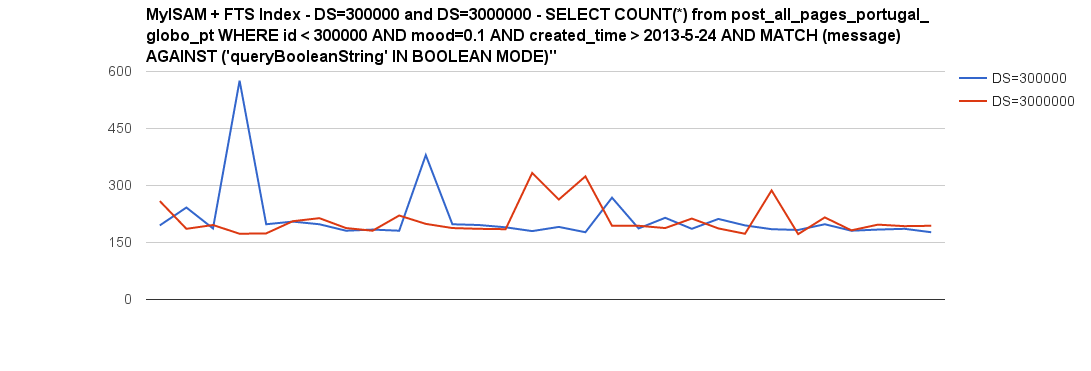
\includegraphics[width=150mm]{Imagens/myISAM-FTSIndex.png}
	\caption{Searching on posts table - New Format: MyISAM and FTS Index \label{fig:myISAM-FTSIndex}}
\end{figure}


\textbf{InnoDB vs MyISAM}

Using MyISAM and a FTS index in MySQL have its downsides, however. As shown on section \ref{classifypostssection}, major features of relational DBs, as \textit{transactional integrity (ACID compliance)} and \textit{foreign keys / cascading deletes},  are lost when using MyISAM engine instead of InnoDB. 

Table locks on MyISAM are also a huge problem, as pointed out by \cite{scoutmigration} (when a table is updated, no other changes to that table can be performed). If the application needed to assure integrity of transactions, for example, engineers would have to do it by their own.

Another possible option is to have two databases - a master (where the updates and ACID compliance operations are done) and a slave (where search operations are done). This approach enables to have all the benefits from InnoDB and MyISAM at the same time. As a downside, however, all the problems of data replication in a master-slave database architecture arise to be handled by the application engineers. 


\textbf{Is MySQL \textit{really} for search?}

Using MATCH AGAINST operator in MyISAM tables have another big downside: the support for \textbf{stemming}.

Stemming, in search, ``\textit{describes the process for reducing inflected (or sometimes derived) words to their word stem, base or root form - generally a written word form}'' \cite{stemming}. A stemming algorithm reduces the words ``playing", ``played'', and ``player'' to the root word, ``play''. ``argue", ``argued'', ``argues'', ``arguing'', and ``argus'' correspond to the stem ``argu'' (a stem is not itself a word or root) but ``argument'' and ``arguments'' are related to the stem ``argument'' \cite{stemming}.

When a user searches for ``lay'' using the LIKE operator, MySQL will return all the posts that contain ``lay'' as a substring. i.e: posts that mention ``play'', ``lay'' and ``laying'' will come as results, which is not what the user expects. On the other hand, when the users search for ``lay'' using the MATCH AGAINST operator, it will only return posts that exactly mention ``lay'', excluding posts that mention ``lays'' or ``layed''. Both results are not what users expect when using popular search tools, like Google.com.

Tickets reffering to the support of stemming were open in 2010 on MySQL's development roadmap \cite{dictionarymysql} \cite{stemmingmysql}. Despite being flagged as ``very high priority'' tasks, they still remains un-assigned for more than 6 years, and even when the support for this operation is eventually released, it will only provide support to english language. 

Possible alternatives to support stemming operations on MySQL would be \textit{i) to build stemming functions on the top of MySQL from the ground up} or \textit{ii) to use external plugins, like \cite{udmstemmer} and \cite{udfstemmer}}. Using external plugins has major downsides, as projects may be discontinued - the last commit on both cited plugins are from 2007 and 2009, respectively, and there's no community support around these technologies. 

Adding support to stemming functions in a database may become a big task, and besides query complexity, it's hard to compete with the performance of a dedicated search engine.   

\textbf{A search engine is needed}

Apache Solr, Lucene, Amazon Cloudsearch and Elasticsearch are \textbf{Search Engines} that provide fulltext-search and Stemming as main features.

After performing extensive literature review, discussing in popular technical forums and analyzing benchmarks \cite{StackOverflowElastic} \cite{SolrVsES} \cite{quoraES}, Elasticsearch (a.k.a. Elastic) seemed to be a good alternative to the problem that the application struggled with MySQL.

On the next section we discuss a new data model to the posts and show how Elasticsearch enabled a \textit{Filter captured posts by filters} operation that runs on a SLA-acceptable level and gives the results that users expect. 

 










\clearpage
\subsection{Map current schema \& data on the proposed DB architecture}

On the last section we discussed how a search engine can help to make the \textit{Filter captured posts by filters} operation run on an acceptable SLA level and deliver the results that users expect from a search operation. 

In this section we detail how using Elasticsearch in a polyglot-persistence approach helped to solve the problems that were found while handling search operations on MySQL.

\textbf{A new data model}

A new data model should be proposed once the new database technology is chosen. As Elasticsearch stores data as JSON documents, the same structure of a post post row on the relational schema was transformed into a valid JSON document.

Listing \ref{post-on-elasticsearch-index} shows how a post row is represented as a JSON document on Elasticsearch indexes. Tags information is stored both as a text field and as an indexed JSON element.

\begin{lstlisting}[language=JSON,firstnumber=1, caption=Post representation - JSON document, label=post-on-elasticsearch-index]

{
   "id": 732632,
   "post_id": 731899886918573,
   "comment_id": 732001700241725,
   "comment_reply_id": 0,
   "fan_page": null,
   "collected_from": "FAN_PAGE",
   "created_time": "2015-06-23T16:51:38.000Z",
   "updated_time": null,
   "message": "Permito-me acreditar mais no cidadao comum do que na autoridade em questao! E isto sera crime? Vamos ver...",
   "type": null,
   "link": null,
   "name": null,
   "caption": null,
   "description": null,
   "picture": null,
   "source": null,
   "mood": 1,
   "icon": null,
   "likes": 12,
   "comments": null,
   "page_id": 144632798978621,
   "group_id": null,
   "page_url": null,
   "author_id": 1131060413576410,
   "author_name": "Nuno Miranda",
   "author_gender": "n",
   "upload": 1,
   "in_reply_to": null,
   "tags": "[{\"name\": \"Adela\", \"user\": \"The\"}, {\"name\": \"Adele\", \"user\": \"functions\"}, {\"name\": \"Adell\", \"user\": \"this\"}, {\"name\": \"Agripina\", \"user\": \"instantiate\"}, {\"name\": \"Adelia\", \"user\": \"each\"}, {\"name\": \"Adena\", \"user\": \"You\"}]",
   "replied_element_id": null,
   "replies": 0,
   "shares": 0,
   "term": null,
   "archived_by_user": null,
   "archived": 1,
   "location": null,
   "tag": [
      {
         "tag_name": "The",
         "tag_user": "Adela"
      },
      {
         "tag_name": "functions",
         "tag_user": "Adele"
      },
      {
         "tag_name": "this",
         "tag_user": "Adell"
      },
      {
         "tag_name": "instantiate",
         "tag_user": "Agripina"
      },
      {
         "tag_name": "each",
         "tag_user": "Adelia"
      },
      {
         "tag_name": "You",
         "tag_user": "Adena"
      }
   ]
}

\end{lstlisting} 


A new server with the same configurations of the one listed on section \ref{appserver} was provisioned and Elasticsearch version 1.7.2 was installed.

The portuguese Language Analyzer \cite{eslanguageanalyzers} for Elasticsearch was also activated to enable stemming and querying user-expected results on portuguese language.

To dump the data from MySQL and import to Elasticsearch, a Python script was made \cite{mysqltoes}. However, loading data was taking too long as the script didn't paralellize the bulk insert queries on Elasticsearch and database connection kept dropping. To overcome this issue, an open-source project that connects Elasticsearch to MySQL via JDBC and imports data \cite{elasticjdbc} was used. 

The mapping from the relational tables to the elasticsearch indexes was done using the transform query presented on Figure \ref{fig:mysql-to-es}.

\begin{figure}[ht!]
	\centering
	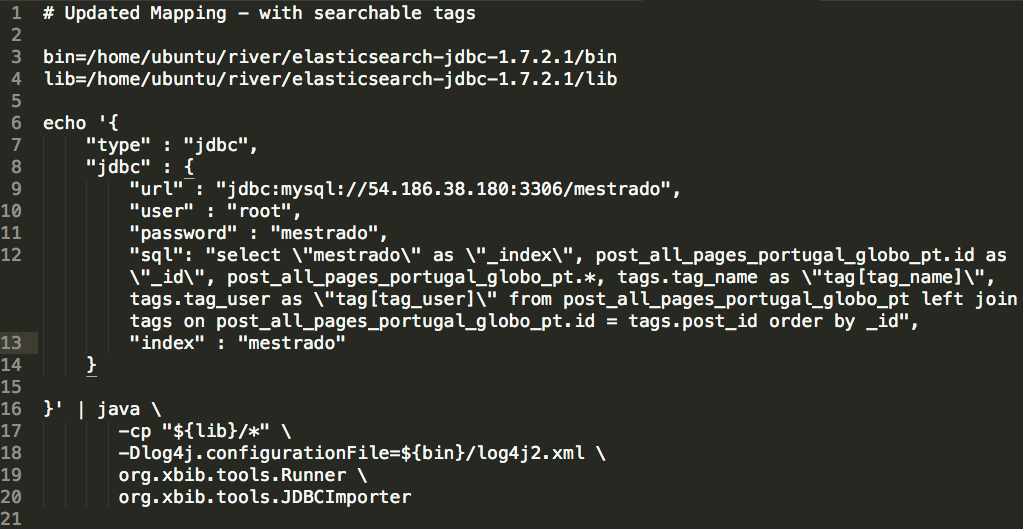
\includegraphics[width=120mm]{Imagens/mysqlToES.png}
	\caption{Mapping - MySQL to ES \label{fig:mysql-to-es}}
\end{figure}

Once the Elasticsearch index was built and the data was successfully imported, the next step of the guidelines should be executed (to process DB operations from a historical point).


\subsection{Process all DB operations from a historical point}

On this step we should execute all operations that were triggering SLA exceptions from the application logs. As this case study built scenarios that represent application logs, the correspondent action would be to run the same operations on the proposed architecture. 

As shown on previous sections, all three operations \textit{(Retrieve posts by id)}, \textit{Classify posts (add/remove tags)} and \textit{Filter captured posts by filters}
satisfied the proposed SLAs when database-level improvements were performed. 

This way, what needs to be done in this step is to verify if the Elasticsearch architecture enables \textit{Filtering captured posts by filters} without triggering any SLA exceptions.

Figures \ref{fig:retrieve-posts by-id-es}, \ref{fig:search-tags} and \ref{fig:es-filters} respectively present the performance of the three operations using the proposed Elasticsearch architecture instead of MySQL. No SLA violations were triggered when performing the operations on the new architecture.

\begin{figure}[ht!]
	\centering
	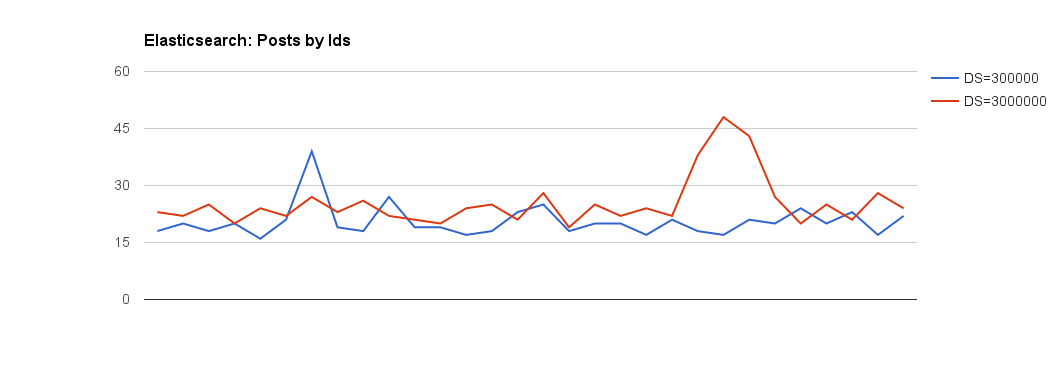
\includegraphics[width=150mm]{Imagens/es-posts-by-ids.png}
	\caption{Elasticsearch architecture: Retrieve posts by Id\label{fig:retrieve-posts by-id-es}}
\end{figure}

\begin{figure}[ht!]
	\centering
	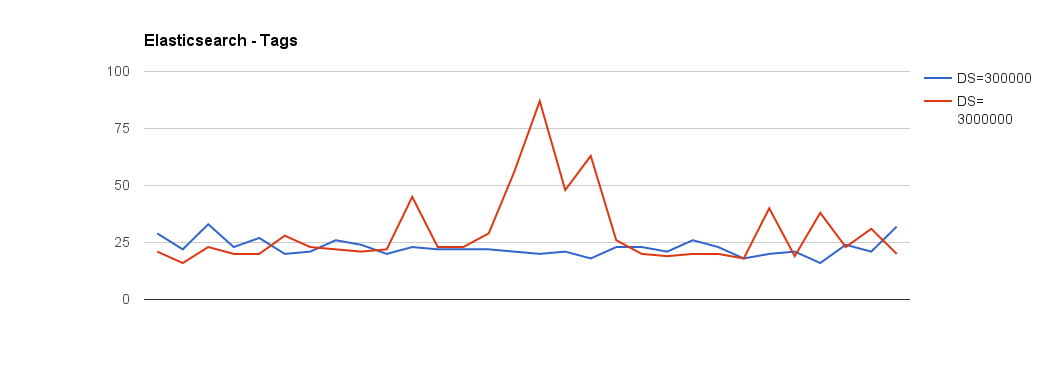
\includegraphics[width=150mm]{Imagens/es-search-tags.png}
	\caption{Elasticsearch architecture: Update by tags \label{fig:search-tags}}
\end{figure}

\begin{figure}[ht!]
	\centering
	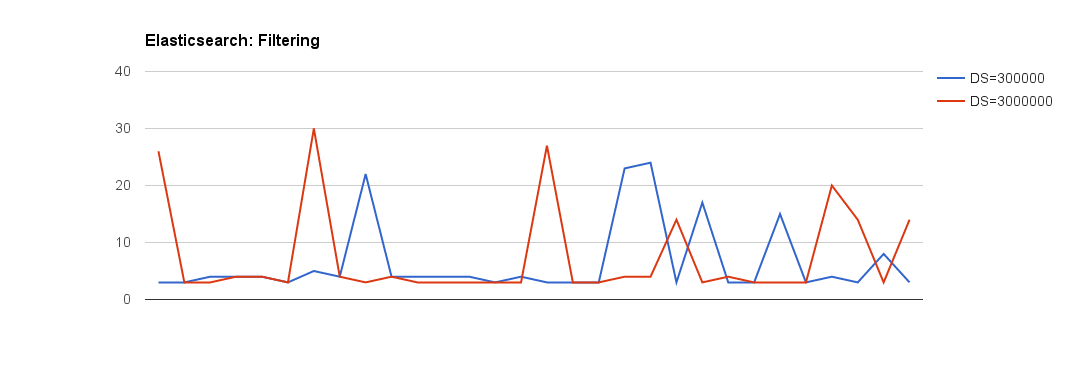
\includegraphics[width=150mm]{Imagens/es-filters.png}
	\caption{Elasticsearch architecture: Filter posts \label{fig:es-filters}}
\end{figure}

Figures \ref{fig:es-query-es-get-posts-by-ids}, \ref{fig:es-query-es-get-tags} and \ref{fig:es-get-filters} show how the three operations can be performed using Elasticsearch query language instead of SQL. 

\begin{figure}[ht!]
	\centering
	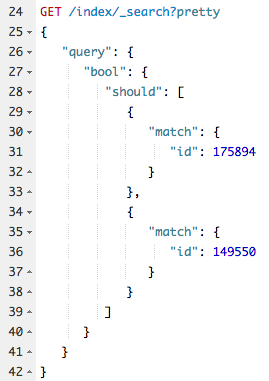
\includegraphics[width=40mm]{Imagens/es-get-posts-by-ids.png}
	\caption{Elasticsearch query: get posts by ids\label{fig:es-query-es-get-posts-by-ids}}
\end{figure}

\begin{figure}[ht!]
	\centering
	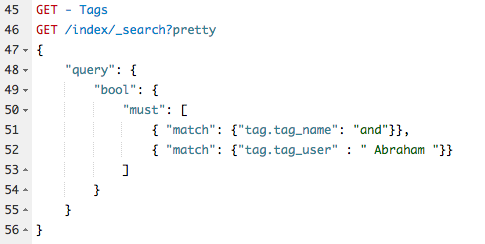
\includegraphics[width=90mm]{Imagens/es-get-tags.png}
	\caption{Elasticsearch query: Posts with tags \label{fig:es-query-es-get-tags}}
\end{figure}


\begin{figure}[ht!]
	\centering
	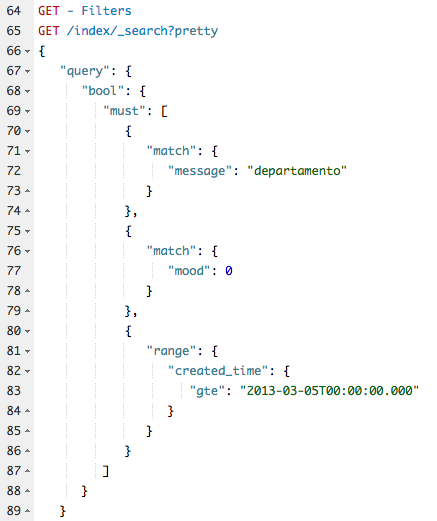
\includegraphics[width=70mm]{Imagens/es-get-filters.png}
	\caption{Elasticsearch query: Filter posts by filters \label{fig:es-get-filters}}
\end{figure}

\subsection{What else elasticsearch enables?}

Besides being able to execute the three operations at a desired QoS, adding a Elasticsearch to the stack of the application enables a number of features that are \textit{technically possible} to have with MySQL, but have poor performance when compared to other NoSQL solutions, as search engines.

An interesting report to have in a social-media monitoring application is a ``word cloud''. In the context of the Facebook component, a word cloud shows the count of terms from the ``message" field. \cite{mysqlstringsplitter} and \cite{mysqlSplitterStoredProcedure} discuss a method of building a word counting system with MySQL. The process relies in having a second table where each word from each ``message'' is inserted and then a COUNT (DISTINCT()) query is performed. 

In the worst case of the proposed scenarios, 3.000.000 posts would have to be analyzed. If the \textit{message} field contains 21 words on average, a word count in this scenario represents a total of 630.00.000 (3.000.000 x 21) INSERTS in a separate table just to count the words. A stored procedure that makes use of this approach is available on \cite{mysqlSplitterStoredProcedure}.

Other way to perform word count using MySQL is to retrieve the posts from the database and perform a programmatic count using parallel processes in several machines, but this approach would also require a high amount of extra effort, as handling with network conditions and woud require extremely high network throughput to deliver results within seconds. 

Concepts as \textit{bucketing}, \textit{in-memory-processing}, \textit{aggregations} and \textit{term-vectors} make the \textit{word-frequency count} job much easier (and near realtime \cite{termVectorsES}) when performed by Search Engines, as Lucene and Elasticsearch, as discussed on \cite{mysqlSplitterStoredProcedure} and fully explained in \cite{termVectorsES}.

Elasticsearch aggregations and filters enable statistics to be delivered in near-realtime even when handling massive datasets \cite{termVectorsES}. This has some other downsides, however. Many of the elasticsearch operations are made at memory level, instead of in-disk. This implies that elasticsearch clusters need high amounts of memory, and applications that rely on elasticsearch must constantly monitor the cluster health to add resources or perform modifications on the documents mappings. Elasticsearch's API to handle with cluster health is available on \cite{clusterHealthES}. 

Several other operations that are simplified by Elasticsearch instead of using MySQL can be named: 
\begin{enumerate}
\item{\textbf{FTS support in several languages:} Performing full-text search in 32 different languages is natively supported by Elasticsearch \cite{eslanguageanalyzers}.}
\item{\textbf{``Did you mean?'' feature:} Operations that suggest corrections to user typos are simplified by using the search term suggester feature on elasticsearch\cite{termsuggester}}
\item{\textbf{Deep paging feature:} On the proposed application architecture (Figure \ref{fig:apparchitecture}), each social network component has its own data storage (MySQL DB). When a user queries for a string term on the interface, it's expected that the application presents the posts (from whatever social network they are from) that match the selected criteria paginated in bulks of X posts. This way, the Adapter component has to perform pagination across multiple data repositories (i.e: Twitter component, Facebook component, Youtube component). 

Supposing that each page that is presented has 10 posts, when a user queries for the last 10 posts, for example, the application has to execute an algorithm that joins the first 10 posts of all databases in a single view. Sorting and paging posts on multiple data repositories are a problematic task, as revealed by \cite{paginationES}.

To understand why deep paging is problematic, suppose that the proposed application has 5 distinct social network components. When the user requests the first page of results (results 1 to 10), each component produces its own top 10 results and returns them to the adapter component, which then sorts all 50 results in order to select the overall top 10.

Now imagine that the user asks for page 1.000 (results 10.001 to 10.010). Everything works in the same way except that each social network component has to produce its top 10.010 results. The adapter component then sorts through all 50.050 results and discards 50.040 of them. That's why, in a distributed system, the cost of sorting results grows exponentially the deeper the page is \cite{paginationES}.

Leaving the pagination task to be done by Elasticsearch removes a potentially problematic business logic from the Adapter component, making the application more maintainable and simple.

}

\end{enumerate}

\subsection{Case study conclusions}
On this chapter we have analyzed how the proposed guidelines can help a software team to assess and execute database-level migrations, transitioning (part of an application) from relational databases to NoSQL architectures.

All operations that were listed on the initial steps of the case study could be performed by the relational database (MySQL), although a series of database-level improvements were needed. 

In a real application it is necessary to analyze the trade-off of \textit{i) making a series of database/source-code improvements to meet the desired QoS} or \textit{ii) adding a new/replacing the database layer of an application.} In some scenarios, improving too much the current database architecture and source code can oftenly lead to hard-to-maintain applications, as related by \cite{scoutmigration}. 

Adding support to multiple databases on an application can help to improve QoS and accelerate application development, but can also be an unnecessary move, as revealed by the sections of this chapter. Each application needs to be extensively analyzed before proposing database-level transitions on production environments. 

One of the main outcomes of the study is to show that \textit{not always} it is necessary to completely switch the data layer from relational databases to NoSQL. As the previous sections proved, architectural changes at relational databases can be made to have similar performance to NoSQL databases in certain scenarios. 

In some scenarios, however, using a NoSQL architecture (as Elasticsearch in the context of this app) can help to leverage user experience, QoS and accelerate application development.  


\textbf{Transition recommendations}

Database transitions, as any refactoring in software projects, should be test-oriented to assure that not only the transitions will bring better QoS, but will also not change the way that the application works. 

Even in tested tests, it's not advisable to completely replace a database at once, as un-tested scenario behaviors may change between databases. In a complete transition scenario, parts of the application can be progressively switched between the data layers to assure that application users will not experience a major fault. 

It's also highly advisable to \textit{verify} if the proposed migration will be able to successfully handle the real workload before using a migrated scenario in production. In other words, it's recommended to run both storage solutions for a while, handling production requests in parallel, ignoring the results of the proposed architecture, to verify that it will be able to successfully handle the workload once the environment is completely transitioned.

It's also advisable to re-visit the recommendations presented on section \ref{transitioning-recommendations} when transitioning a real application. These recommendations were extracted from a set of industry reports from migration scenarios and are also part of the proposed guidelines.
